\documentclass{magnoliaold}

\magtex{tex_driver={pdftex},
        tex_packages={epigraph,xypic}}
\magfiche{document_nom={Fonctions usuelles},
          auteur_nom={François Fayard},
          auteur_mail={fayard.prof@gmail.com}}
\magcours{cours_matiere={maths},
          cours_niveau={mpsi},
          cours_chapitre_numero={3},
          cours_chapitre={Fonctions usuelles}}
\magmisenpage{misenpage_presentation={tikzvelvia},
          misenpage_format={a4},
          misenpage_nbcolonnes={1},
          misenpage_preuve={non},
          misenpage_sol={non}}
\maglieudiff{}
\magprocess

\begin{document}

%BEGIN_BOOK
\setlength\epigraphwidth{.6\textwidth}
\epigraph{\og En mathématiques, on ne comprend pas les choses, on s’y habitue.\fg}{--- \textsc{John Von Neumann (1903--1957)}}
\setlength\epigraphwidth{.5\textwidth}
\epigraph{\og Le logarithme de \nom{John Napier}, en réduisant leur travail, a doublé la vie des astronomes.\fg}{--- \textsc{Pierre-Simon Laplace (1749--1827)}}
\setlength\epigraphwidth{.3\textwidth}
\epigraph{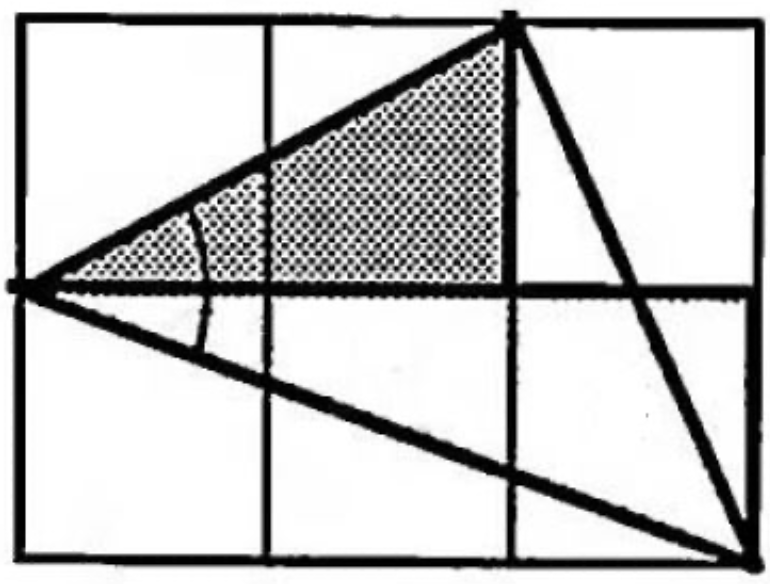
\includegraphics[width=0.9\textwidth]{../../Commun/Images/maths-cours-machin.png}\\
\og $\arctan\frac{1}{2}+\arctan\frac{1}{3}=\frac{\pi}{4}.$ \fg}{--- \textsc{Leonhard Euler (1707--1783)}}

\magtoc

\section{Logarithme, exponentielle, puissance}
\subsection{Logarithme népérien}
\begin{definition}[utile=-3]
On appelle \emph{logarithme népérien} et on note $\ln$ l'unique primitive sur $\RPs$ de la fonction $x\mapsto 1/x$ qui s'annule en~1.
\[\dspappli{\ln}{\RPs}{\R}{x}{\integinv{1}{x}{t}{t}}\]
\end{definition}

\begin{remarqueUnique}
\remarque Le nom $\ln$ est à la fois l'acronyme de logarithme naturel et de
  logarithme népérien (en hommage à \nom{John Napier}, mathématicien Écossais,
  1550--1617).
\end{remarqueUnique}

\begin{proposition}[utile=-3]
\begin{itemize}
\item $\ln$ est continue sur $\RPs$.
\item $\ln$ est dérivable sur $\RPs$ et
  \[\forall x\in\RPs \qsep \ln' x=\frac{1}{x}.\]
% \item $\ln$ est $\classec{\infty}$ sur $\RPs$.
\end{itemize}
\end{proposition}

\begin{preuve}
Tout vient de la définition précédente.
\end{preuve}

\begin{remarqueUnique}
\remarque La fonction
  \[\dspappli{f}{\Rs}{\R}{x}{\ln\abs{x}}\]
  est dérivable sur $\Rs$ et, pour tout $x\in\Rs$, $f'(x)=1/x$. Autrement dit, sur $\Rs$
  \[\priminv{x}{x}=\ln\abs{x}.\]
\end{remarqueUnique}

\begin{proposition}[utile=-3]
\begin{eqnarray*}
                   & & \ln 1=0,\\
\forall x,y\in\RPs, & & \ln\p{xy}=\ln x+\ln y,\\
\forall x\in\RPs, & & \ln\p{1/x}=-\ln x,\\
\forall x\in\RPs \qsep \forall n\in\Z, & & \ln x^n=n\ln x.
\end{eqnarray*}
\end{proposition}

\begin{preuve}
On définit $\dspappli{\varphi}{\RPs}{\R}{y}{\ln(xy)-\ln(x)-\ln(y)}$ et on montre que $\varphi$ est nulle en la dérivant.
La suite en découle.
\end{preuve}

\begin{proposition}[utile=-3]
\[\forall x\in\RPs \qsep \forall n\in\Ns \qsep
  \ln\sqrt[n]{x}=\frac{1}{n}\cdot\ln x.\]
\end{proposition}

\begin{proposition}[utile=-3]
$\ln$ est strictement croissante sur $\RPs$. De plus
\[\ln x \tendvers{x}{+\infty} +\infty \et
  \ln x \tendvers{x}{0} -\infty.\]
\end{proposition}

\begin{preuve}
$\ln$ admet une limite dans $\overline{\R}$. Il suffit alors de montrer qu'elle n'est pas majorée, ce qu'on peut faire, via $\ln(2^n)=n\ln(2)$.

$\ln(x)=-\ln(1/x)$ pour l'autre.
\end{preuve}
\begin{exoUnique}
\exemple Résoudre l'inéquation $\ln\abs{x+1}-\ln\abs{2x+1}\leq\ln 2$.
  \begin{sol}
On réunit tous les $\ln$ du même côté puis on enlève les log puis on élève au carré (par équivalence) et on obtient $x\in\interof{-\infty}{-3/5}\cup\interfo{-1/3}{+\infty}$. 
  \end{sol}
\end{exoUnique}

\begin{proposition}[utile=-3]
$\ln$ réalise une bijection de $\RPs$ dans $\R$.
\end{proposition}

\begin{preuve}
limites + stricte croissance.
\end{preuve}

\begin{definition}[utile=-3]
Il existe un unique réel, noté $\e$ et appelé \emph{nombre de \nom{Néper}}, tel que $\ln \e=1$.
\end{definition}



\begin{preuve}
$n\ln\sqrt[n]{x}=\ln\p{\p{\sqrt[n]{x}}^{n}}=\ln(x)$.
\end{preuve}


\begin{proposition}[utile=-3]
\[\forall x\in\intero{-1}{+\infty} \qsep \ln\p{1+x}\leq x.\]  
\end{proposition}

\begin{preuve}
Simple étude de fonction.
\end{preuve}


\begin{exoUnique}
\exemple Montrer que pour tout $n\in\Ns$,
  $\frac{1}{n+1}\leq\ln\p{1+\frac{1}{n}}\leq\frac{1}{n}$.
\end{exoUnique}

\begin{sol}
\nom{Victor}~: $\ln\p{1+\frac{1}{n}}=\ln(n+1)-\ln(n)$ qu'on voit comme une intégrale qu'on encadre.\\
\nom{François}~: Soit $n\in\Ns$. Alors
\[\ln\p{1+\frac{1}{n}}\leq\frac{1}{n}\]
d'après la proposition précédente. Pour la première inégalité, on a
\[\ln\p{1+\frac{1}{n}}=\ln\p{\frac{n+1}{n}}=-\ln\p{\frac{n}{n+1}}=-\ln\p{1-\frac{1}{n+1}}.\]
Or, en utilisant la proposition précédente
\[\ln\p{1-\frac{1}{n+1}}\leq -\frac{1}{n+1}\]
donc
\[\ln\p{1+\frac{1}{n}}\geq\frac{1}{n+1}.\]
\end{sol}

\begin{proposition}[utile=-3]
\[\frac{x}{\ln x}\tendvers{x}{+\infty} +\infty, \qquad
  x\ln x\tendvers{x}{0} 0,\]
\[\frac{\ln\p{1+x}}{x} \tendvers{x}{0} 1.\]  
\end{proposition}

\begin{preuve}
$\ln(u)\leq u$ appliqué en $\sqrt{x}$ donne $\frac{\ln x}{x}\tendvers{x}{+\infty} 0$ par valeur supérieure.

$x\ln(x)=-\dfrac{\ln(1/x)}{1/x}$ permet de conclure pour la deuxième limite.

Taux d'accroissement pour la dernière.

\end{preuve}

\begin{center}
\begin{pdfpic}
\readdata{\listePln}{graph/graphe_ln.txt}
\psset{xunit=2.3cm,yunit=2.3cm}
\begin{pspicture}(-1,-2.2)(4.2,1.6)
  \psaxes[labels=none]{->}(0,0)(-1,-2.2)(4.2,1.6)
  \dataplot[plotstyle=curve,linewidth=2pt]{\listePln}
  \psline[linewidth=0.5pt](-0.8,-1.8)(2.38,1.38)
  \uput[ul](2,1){$y=x-1$}
  \uput[d](1,0){1}
  \uput[d](2.718,0){${\rm e}$}
  \psline[linestyle=dashed,linewidth=0.5pt](2.718,0)(2.718,1)
  \psline[linestyle=dashed,linewidth=0.5pt](2.718,1)(0,1)
  \uput[l](0,1){1}
  \uput[r](4.2,0){$x$}
  \uput[r](0,1.6){$y$}
  \uput[dr](3.2,1.163){$y=\ln x$}
\end{pspicture}
\end{pdfpic}
\end{center}


\subsection{Exponentielle}

\begin{definition}[utile=-3]
Pour tout $y\in\R$, il existe un unique $x\in\RPs$ tel que $\ln x=y$; on le
note $\exp y$. On définit ainsi la fonction
\[\dspappli{\exp}{\R}{\RPs}{y}{\exp y.}\]
\end{definition}

\begin{remarques}
\remarque Autrement dit, $\exp$ est la bijection réciproque de $\ln$.
\remarque Par définition
  \[\forall x\in\R\qsep \exp x>0.\]
\end{remarques}

\begin{proposition}[utile=-3]
\begin{eqnarray*}
\forall x\in\R, & & \ln\p{\exp x}=x,\\
\forall x\in\RPs, & & \exp\p{\ln x}=x.    
\end{eqnarray*}
\end{proposition}

\begin{proposition}[utile=-3]
$\exp$ réalise une bijection de $\R$ dans $\RPs$.
\end{proposition}

\begin{proposition}[utile=-3]
\begin{eqnarray*}
\exp 0=1, & & \exp 1=\e,\\
\forall x,y\in\R, & & \exp\p{x+y}=\exp(x)\exp(y),\\
\forall x\in\R, & & \exp\p{-x}=\frac{1}{\exp x},\\
\forall x\in\R \qsep \forall n\in\Z, & & \exp\p{nx}=\p{\exp x}^n.
\end{eqnarray*}
\end{proposition}

\begin{preuve}
$\exp(x+y)=\exp(\ln(\exp(x))+\ln(\exp(y)))$...
\end{preuve}

\begin{proposition}[utile=-3]
$\exp$ est strictement croissante sur $\R$. De plus
\[\exp x\tendvers{x}{-\infty} 0 \et \exp x\tendvers{x}{+\infty} +\infty.\]
\end{proposition}

\begin{preuve}
Croissante par bijection réciproque d'une fonction croissante et les limites car elle est bijective.
\end{preuve}


\begin{proposition}[utile=-3]
\begin{itemize}
\item $\exp$ est continue sur $\R$.
\item $\exp$ est dérivable sur $\R$ et
  \[\forall x\in\R \qsep \exp' x=\exp x.\]
% \item $\exp$ est $\classec{\infty}$ sur $\R$.
\end{itemize}
\end{proposition}

\begin{preuve}
$f$ bijective et dérivable telle que $f'$ ne s'annule pas sur $I$, alors $f^{-1}$ est dérivable sur $I$ et $(f^{-1})'=1/(f'\circ f^{-1})$.
\end{preuve}

\begin{proposition}[utile=-3]
\[\forall x\in\R \qsep \exp x \geq 1+x.\]
\end{proposition}
\begin{preuve}
Si $x\leq -1, 1+x\leq 0 \leq \exp x$. Sinon, $\ln(1+x)\leq  x$ puis passage à l'exponentielle.
\end{preuve}

\begin{exos}
\exemple Montrer que
  \[\forall x<1 \qsep \exp x\leq\frac{1}{1-x}.\]
  \begin{sol}
  $\forall x\in\R \qsep \exp (-x) \geq 1-x.$ Si $x<1$, $1-x>0$ et par décroissance de la fonction inverse sur $\RPs$, on a le résultat.
  \end{sol}
\exemple Soit $a,b\in\R$ tels que $0<a<b$. Montrer que
  \[\forall x\in\RPs \qsep 0<b\exp(-ax)-a\exp(-bx)<b-a.\]
  \begin{sol}
  On dérive la fonction à l'intérieur. Elle est décroissante, vaut $b-a$ en $0$ et sa limite en l'infini est $0$.
  \end{sol}
\end{exos}

\begin{proposition}[utile=-3]
\[\frac{\exp x}{x} \tendvers{x}{+\infty} +\infty, \qquad
  x\exp x \tendvers{x}{-\infty} 0,\]
\[\frac{\exp(x)-1}{x} \tendvers{x}{0} 1.\]
\end{proposition}

\begin{preuve}
 On peut poser $x=\ln u$ et se ramener à la limite de $u/\ln(u)$ en $+\infty$.

$x\exp(x)=-x/\exp(-x)$ permet d'avoir la deuxième limite.

Taux d'accroissement pour la troisième.
\end{preuve}

\begin{center}
\begin{pdfpic}
\readdata{\listePln}{graph/graphe_ln.txt}
\readdata{\listePexp}{graph/graphe_exp.txt}
\psset{xunit=1.8cm,yunit=1.8cm}
\begin{pspicture}(-2.2,-2.2)(4.2,4.2)
  \psaxes[labels=none]{->}(0,0)(-2.2,-2.2)(4.2,4.2)
  \dataplot[plotstyle=curve,linestyle=dashed,linewidth=0.5pt]{\listePln}
  \dataplot[plotstyle=curve,linewidth=2pt]{\listePexp}
  \uput[d](1,0){1}
  \uput[l](0,2.718){${\rm e}$}
  \psline[linestyle=dashed,linewidth=0.5pt](0,2.718)(1,2.718)
  \psline[linestyle=dashed,linewidth=0.5pt](1,2.718)(1,0)
  \psline[linewidth=0.5pt](-2,-2)(4,4)
  \psline[linewidth=0.5pt](-2,-1)(3,4)
  \uput[l](0,1){1}
  \uput[r](4.2,0){$x$}
  \uput[r](0,4.2){$y$}
  \uput[dr](3.2,1.163){$y=\ln x$}
  \uput[r](1.2527,3.5){$y=\exp x$}
  \uput[r](1,2){$y=x+1$}
  \uput[dr](3,3){$y=x$}
\end{pspicture}
\end{pdfpic}
\end{center}

\subsection{Logarithme et exponentielle en base $a$}

\begin{definition}[utile=-3]
Soit $a\in\RPs\setminus\ens{1}$. On appelle \emph{logarithme en base $a$} et on note
$\log_a$ la fonction
\[\dspappli{\log_a}{\RPs}{\R}{x}{\frac{\ln x}{\ln a}.}\]
\end{definition}

\begin{remarqueUnique}
\remarque Le logarithme népérien est le logarithme en base
  $\e$. Si $a=10$, on obtient le logarithme décimal qui est utilisé  en
  physique (pour définir les décibels) et en chimie (pour définir le pH).% Enfin, si $a=2$, on obtient le
%  logarithme binaire, utilisé en informatique.
%\remarque En \verb+Maple+, les fonctions \verb+ln+ et \verb+log+ font toutes
%  les deux référence au logarithme népérien. Pour obtenir le logarithme de $x$
%  en base $a$, on utilisera la commande \verb+log[a](x)+. Enfin, la fonction
%  \verb+log10+ fait référence au logarithme en base 10.
\end{remarqueUnique}

\begin{exoUnique}
\exo Résoudre le système
  \[\begin{cases}
    2\log_x y+2\log_y x=-5 &\\
    xy=\e. &
    \end{cases}\]
  \begin{sol}
  On remplace $x$ ou $y$ grâce à la deuxième équation puis on pose $u=\ln(y)/(1-\ln(y))$. On obtient $u=-2$ ou $u=-1/2$ donc on trouve $x=e^2$ et $y=1/e$ et inversement.    
  \end{sol}
\end{exoUnique}

\begin{proposition}[utile=-3]
Soit $a\in\RPs\setminus\ens{1}$. Alors
\begin{eqnarray*}
\forall x,y\in\RPs, & & \log_a \p{xy}=\log_a  x+\log_a  y,\\
\forall x\in\RPs, & & \log_a \p{1/x}=-\log_a  x,\\
\forall x\in\RPs \qsep \forall n\in\Z, & & \log_a  x^n=n\log_a x.
\end{eqnarray*}
\end{proposition}

\begin{definition}[utile=-3]
Soit $a\in\RPs\setminus\ens{1}$. Alors, pour tout $y\in\R$, il existe un unique
$x\in\RPs$ tel que $\log_a x=y$; on le note $\exp_a y$ et on a
\[\exp_a y=\exp\p{y\ln a}.\]
On définit ainsi la fonction
\[\dspappli{\exp_a}{\R}{\RPs}{y}{\exp\p{y \ln a .}}\]
\end{definition}

\begin{remarqueUnique}
\remarque Lorsque $a=\e$, on retrouve la fonction exponentielle.  
\end{remarqueUnique}

% \begin{proposition}[utile=-3]
% Soit $a\in\RPs\setminus\ens{1}$. Alors
% \begin{eqnarray*}
% \exp_a  0=1 & & \exp_a  1=a\\
% \forall x,y\in\R & & \exp_a \p{x+y}=\exp_a (x)\exp_a (y)\\
% \forall x\in\R & & \exp_a \p{-x}=\frac{1}{\exp_a  x}\\
% \forall x\in\R \qsep \forall n\in\Z & & \exp_a \p{nx}=\p{\exp_a  x}^n
% \end{eqnarray*}
% \end{proposition}

\subsection{Fonction puissance}

\begin{definition}[utile=-3]
Pour $x\in\RPs$ et $y\in\R$, on définit $x^y$ par
\[x^y\defeq\exp\p{y \ln x}.\]
\end{definition}

\begin{remarques}
\remarque En particulier, pour tout $x\in\R$, $\exp x=\e^x$. Plus généralement,
   si $a\in\RPs\setminus\ens{1}$
   \[\forall x\in\R \qsep \exp_a(x)=a^x.\]
   On utilisera désormais cette notation pour désigner l'exponentielle ainsi que
   l'exponentielle en base $a$.
\remarque Afin de dériver une fonction de la forme $f(x)\defeq u(x)^{v(x)}$, il est recommandé de la mettre sous la forme
  \[f(x)=\e^{v(x)\ln\p{u(x)}}.\]
\end{remarques}

\begin{exos}
\exemple Résoudre l'équation $x^{\sqrt{x}}=\sqrt{x}^{\ x}$.
  \begin{sol}
  Les solutions de cette équation sont 1 et 4.
  \end{sol}
\exemple Calculer $\fracd{}{x}\p{x^x}$.
  \begin{sol}
  On trouve $\p{\ln x+1}x^x$.
  \end{sol}
\end{exos}

\begin{definition}[utile=-3]
Soit $a\in\R$. On appelle fonction puissance, la fonction définie sur $\RPs$
\[\dspappli{\phi_a}{\RPs}{\R}{x}{x^a .}\]
\end{definition}

\begin{proposition}[utile=-3]
\begin{eqnarray*}
\forall x\in\RPs \qsep x^0=1, & & \forall a\in\R \qsep 1^a=1,\\
\forall x\in\RPs \qsep \forall a,b\in\R, & & x^{a+b}=x^a x^b,\\
\forall x\in\RPs \qsep \forall a\in\R, & & x^{-a}=1/x^a,\\
\forall x,y\in\RPs \qsep \forall a\in\R, & & \p{xy}^a=x^a y^a,\\
\forall x\in\RPs \qsep \forall a,b\in\R, & & \p{x^a}^b=x^{ab},\\
\forall x\in\RPs \qsep \forall a\in\R, & & \ln\p{x^a}=a\ln x .
\end{eqnarray*}
\end{proposition}

\begin{proposition}[utile=-3]
Soit $a\in\R$. La fonction $\phi_a:x\mapsto x^a$ définie sur $\RPs$ est
\begin{itemize}
\item continue sur $\RPs$.
\item dérivable sur $\RPs$ et
  \[\forall x\in\RPs \qsep \phi_a'(x)=a x^{a-1}.\]
% \item $\classec{\infty}$ sur $\RPs$.
\end{itemize}
\end{proposition}

% \begin{remarques}
% \remarque Soit $f_1,\ldots,f_n$ des fonctions dérivables à valeurs
%   strictement positives sur $\mathcal{D}$ et $\alpha_1,\ldots,\alpha_n\in\R$.
%   On définit la fonction $f$ sur $\mathcal{D}$ par
%   \[\forall x\in\mathcal{D} \qsep f(x)=f_1(x)^{\alpha_1}\cdots
%     f_n(x)^{\alpha_n}\]
%   Alors $f$ est dérivable sur $\mathcal{D}$ et
%   \[\forall x\in\mathcal{D} \qsep \frac{f'(x)}{f(x)}=
%     \alpha_1\cdot\frac{f_1'(x)}{f_1(x)}+\cdots+\alpha_n\cdot
%     \frac{f_n'(x)}{f_n(x)}\]
%   Cette relation reste vraie si l'on suppose juste que les fonctions $f_k$
%   sont dérivables et ne s'annulent pas, dans le cas bien sur où l'expression
%   $f_1(x)^{\alpha_1}\cdots f_n(x)^{\alpha_n}$ conserve un sens (c'est-à-dire
%   lorsque les $\alpha_k$ associés aux fonctions $f_k$ prenant des valeurs
%   strictement négatives sont entiers). On a donc
%   \[\forall x\in\mathcal{D} \qsep f'(x)=\sum_{k=1}^n \alpha_k \cdot
%     f_1(x)^{\alpha_1}\cdots f_k'(x)f_k^{\alpha_k-1}(x)\cdots f_n(x)^{\alpha_n}\]
%   Cette relation reste d'ailleurs vraie si l'on suppose juste les fonctions
%   $f_k$ dérivables dans la mesure où l'expression $f_1(x)^{\alpha_1}\cdots
%   f_n(x)^{\alpha_n}$ conserve un sens (c'est-à-dire lorsque les $\alpha_k$
%   associés aux fonctions $f_k$ pouvant s'annuler sont entiers naturels).
% \end{remarques}

% \begin{exos}
% \exemple Calculer
%   \[\fracd{}{x}\p{\frac{e^x}{\sqrt{1+x^2}}}, \qquad \fracd{}{x}\p{
%     \frac{x+2}{\sqrt[3]{1+x^2}}}.\]
% \end{exos}

\begin{proposition}[utile=-3]
Soit $a\in\R$. Alors
\[x^a \tendvers{x}{+\infty}
  \begin{cases}
  +\infty & \text{si $a>0$}\\
  1 & \text{si $a=0$}\\
  0 & \text{si $a<0$}
  \end{cases} \et
  x^a \tendvers{x}{0}
  \begin{cases}
  0 & \text{si $a>0$}\\
  1 & \text{si $a=0$}\\
  +\infty & \text{si $a<0$.}
  \end{cases}\]
\end{proposition}


\begin{remarqueUnique}
\remarque Si $a>0$, on définit $0^a$ en posant $0^a\defeq 0$. La fonction
  \[\dspappli{\phi_a}{\RP}{\R}{x}{x^a}\]
  est continue sur $\RP$ et dérivable sur
  \begin{itemize}
  \item $\RP$ lorsque $a\geq 1$ avec
    \[\forall x\in\RP \qsep \phi_a'(x)=a x^{a-1}.\]
  \item $\RPs$ lorsque $a<1$ avec
    \[\forall x\in\RPs \qsep \phi_a'(x)=a x^{a-1}.\]
  \end{itemize}
\end{remarqueUnique}

\begin{center}
\begin{pdfpic}
\readdata{\listePpuissa}{graph/graphe_puissa.txt}
\readdata{\listePpuissb}{graph/graphe_puissb.txt}
\readdata{\listePpuissc}{graph/graphe_puissc.txt}
\readdata{\listePpuissd}{graph/graphe_puissd.txt}
\readdata{\listePpuisse}{graph/graphe_puisse.txt}
\psset{xunit=4cm,yunit=4cm}
\begin{pspicture}(-0.2,-0.2)(2.2,2.2)
  \psaxes[labels=none]{->}(0,0)(-0.2,-0.2)(2.2,2.2)
  \dataplot[plotstyle=curve,linewidth=2pt]{\listePpuissa}
  % \dataplot[plotstyle=curve,linewidth=2pt]{\listePpuissb}
  \dataplot[plotstyle=curve,linewidth=2pt]{\listePpuissc}
  \dataplot[plotstyle=curve,linewidth=2pt]{\listePpuissd}
  \dataplot[plotstyle=curve,linewidth=2pt]{\listePpuisse}
  \psline[linewidth=2pt](0,1)(2,1)
  \uput[r](2.2,0){$x$}
  \uput[r](0,2.2){$y$}
  \uput[dr](1.8,0.5){$y=x^{-1}=1/x$}
  \uput[dr](1.8,1){$y=x^0=1$}
  \uput[ur](1.8,1.25){$y=x^{\frac{1}{3}}=\sqrt[3]{x}$}
  \uput[dr](1.8,1.8){$y=x$}
  \uput[r](1.26,2){$y=x^3$}
  \uput[d](1,0){1}
  \uput[l](0,1){1}
\end{pspicture}
\end{pdfpic}
\end{center}

\begin{proposition}
  \[\forall n\in\Ns\qsep \forall x\geq 0\qsep \sqrt[n]{x}=x^{\frac{1}{n}}.\]
\end{proposition}

\subsection{Calcul de limite}
\begin{proposition}[utile=-3, nom={Croissances comparées}]
Soit $\alpha,\beta>0$ et $n\in\Ns$. Alors
\[\frac{\e^{\alpha x}}{x^\beta}\tendvers{x}{+\infty} +\infty, \qquad
  \frac{x^\alpha}{\p{\ln x}^\beta}\tendvers{x}{+\infty} +\infty,\]
\[x^\alpha \p{\ln x}^n \tendvers{x}{0} 0.\]
\end{proposition}

\begin{preuve}
$\dfrac{e^{\alpha x}}{x^\beta}=\p{\dfrac{e^{\alpha x/\beta}}{x}}^{\beta}=\p{\dfrac{\alpha}{\beta}}^{\beta}.\p{\dfrac{e^{\alpha x/\beta}}{\alpha x/\beta}}^{\beta}$.

$\dfrac{x^\alpha}{\p{\ln x}^\beta}=\p{\dfrac{x^{\alpha/\beta}}{\ln(x)}}^\beta=\p{\dfrac{\alpha}{\beta}}^\beta\p{\dfrac{x^{\alpha/\beta}}{\ln(x^{\alpha/\beta})}}^\beta$.

$x^\alpha \p{\ln x}^n=\p{x^{\alpha/n}\ln(x)}^n=\p{x^{\alpha/n}\ln(x^{\alpha/n})}^n.\p{\dfrac{n}{\alpha}}^n$.
\end{preuve}

\begin{remarques}
\remarque Mnémotechniquement, on dit qu'en 0 et en $+\infty$, l'exponentielle
  l'emporte sur la puissance qui l'emporte sur le logarithme.
\remarque La technique essentielle dans le calcul des limites est la
  \emph{factorisation par le terme principal}~: lorsqu'on fait face à une somme de termes
  qui tendent vers $\pm\infty$, il est nécessaire de factoriser par le terme qui tend
  \og le plus vite vers l'infini\fg. 
\begin{itemize}
\item Pour calculer la limite en $\pm\infty$ des polynômes, il convient de
  factoriser par le monôme de plus haut degré. Par exemple
  $$2x^3-x^2+1=x^3\p{2-\frac{1}{x}+\frac{1}{x^3}}\tendvers{x}{+\infty}+\infty.$$
\item Pour calculer la limite en $\pm\infty$ des fractions rationnelles, il
  convient de factoriser au numérateur et au dénominateur par le monôme de
  plus haut degré. Par exemple
  
 $$\frac{x^2+2x-3}{2x^2-1}=\frac{1+\frac{2}{x}-\frac{3}{x^2}}
                           {2-\frac{1}{x^2}}\tendvers{x}{+\infty}\frac{1}{2}.$$
\item Pour calculer la limite en $\pm\infty$ des fractions rationnelles en $x$
  et en $\e^x$, il convient d'utiliser les croissances comparées en se
  rappelant que l'exponentielle l'emporte sur les puissances
  en $-\infty$ et en $+\infty$. Par exemple
  \[\e^x-x^5=\e^x\p{1-\frac{x^5}{\e^x}}\tendvers{x}{+\infty} +\infty, \qquad
    \frac{\e^{2x}-2x\e^x}{x^3+3\e^{2x}}=\frac{1-2\frac{x}{\e^x}}
    {3+\frac{x^3}{\e^{2x}}}\tendvers{x}{+\infty}\frac{1}{3}.\]
\item Pour calculer la limite en $+\infty$ ou en $0$ des fractions rationnelles
  en $\ln x,x$ et $\e^x$, il convient d'utiliser les croissances comparées en se
  rappelant que l'exponentielle l'emporte sur les puissances
  qui l'emportent sur le logarithme que ce soit en $+\infty$ ou en $0$.
  % Par exemple
  % $$\frac{\e^x\ln x-x^{1000}+\e^{2x}}{\e^{2x}+\ln x+x}=
  %   \frac{1+\frac{\ln x}{\e^x}-\frac{x^{1000}}{\e^{2x}}}
  %        {1+\frac{\ln x}{\e^{2x}}+\frac{x}{\e^{2x}}}\tendvers{x}{+\infty} 1$$
  % \begin{equation*}
  % \begin{split}
  % \frac{x^3\ln x-x^2\ln^2 x}{x+x\ln x}&=-\frac{x^2\ln^2 x}{x\ln x}\cdot
  %                                \frac{1-\frac{x}{\ln x}}{1+\frac{1}{\ln x}}\\
  %                 &=-\p{x\ln x}\frac{1-\frac{x}{\ln x}}{1+\frac{1}{\ln x}}
  %                   \tendvers{x}{0} 0.
  % \end{split}
  % \end{equation*}
\end{itemize}
\remarque Une autre technique importante est la technique du \emph{changement de variable}. Elle
se base sur le théorème de composition des limites. Le principe en est le suivant.
Étant donné une fonction $f$ définie
au voisinage de $a$, on cherche deux fonctions $g$ et $\bar{u}$ telles que sur
ce voisinage
$$f(x)=g(\bar{u}(x)).$$
Si on connait la limite $l$ de $\bar{u}(x)$ lorsque $x$ tend vers $a$ et la
limite $l'$ de $g(u)$ lorsque $u$ tend vers $l$, alors le théorème de
composition des limites permet de conclure que $f(x)$ tend vers $l'$ lorsque $x$ tend vers $a$.
\end{remarques}








% Une autre technique importante est la technique du \emph{changement de variable}. Elle
% se base sur le théorème de composition des limites. Le principe en est le suivant.
% Étant donné une fonction $f$ définie
% au voisinage de $a$, on cherche deux fonctions $g$ et $\bar{u}$ telles que sur
% ce voisinage
% $$f(x)=g(\bar{u}(x)).$$
% Si on connait la limite $l$ de $\bar{u}(x)$ lorsque $x$ tend vers $a$ et la
% limite $l'$ de $g(u)$ lorsque $u$ tend vers $l$, alors le théorème de
% composition des limites permet de conclure que $f(x)$ tend vers $l'$ lorsque $x$ tend vers $a$.

\begin{exos}
% \item On cherche la limite, si elle existe, de
%   $$\frac{\e^{\e^x}}{x^2}.$$
%   lorsque $x$ tend vers $+\infty$.
%   \begin{sol}
%   On pose $u=\e^x$, donc $x=\ln u$.
%     On a alors~:
%     $$\frac{\e^{\e^x}}{x^2}=\frac{\e^u}{\ln^2 u}.$$
%     Or $u$ tend vers $+\infty$ lorsque $x$ tend vers $+\infty$ et les théorèmes
%     de croissances comparées affirment que $\ln^{-2} u\,\e^u$ tend vers
%     $+\infty$ lorsque $u$ tend vers $+\infty$. On en déduit donc que
%     $$\frac{\e^{\e^x}}{x^2}\tendvers{x}{+\infty}+\infty.$$
%     \end{sol}
% \exo Calculer les limites des expressions suivantes.
%   \[2x^3-x^2+1 \quad\text{en $-\infty$}, \qquad
%     \frac{x^2+2x-3}{2x^2-1} \quad\text{en $-\infty$}.\]
%     \begin{sol}
%     On a
%     \[2x^3-x^2+1=2x^3\left(1-\frac{1}{2x}+\frac{1}{2x^{3}} \right)\tendvers{x}{+\infty}+\infty\]
%     \[\frac{x^2+2x-3}{2x^2-1}=\frac{1+\frac{2}{x}-\frac{3}{x^{2}}}{2\left( 1-\frac{1}{2x^{2}}\right) }\tendvers{x}{+\infty}\frac{1}{2}.\]
%     \end{sol}
\exo Calculer la limite de
  % \[\e^x-x^5 \quad\text{en $+\infty$}, \qquad
  \[\frac{\e^x\ln x-x^{1000}+\e^{2x}}{\e^{2x}+\ln x+x}
    \quad\text{en $+\infty$}.\]
    \begin{sol}
    On a
\[\e^x-x^5=\e^x\left( 1-\frac{x^5}{\e^{x}}\right)\tendvers{x}{+\infty} +\infty\]
\[\frac{\e^x\ln x-x^{1000}+\e^{2x}}{\e^{2x}+\ln x+x} = \frac{\frac{\ln x}{\e^{x}}-\frac{x^{1000}}{\e^{2x}}+1}{1+\frac{\ln x}{\e^{2x}}+\frac{x}{\e^{2x}}}\tendvers{x}{+\infty} 1\]
    \end{sol}
\exo Calculer les limites suivantes
\[\frac{(\ln x)^2}{\e^x} \quad \text{en $+\infty$}, \qquad
  \frac{1}{x}\cdot \e^{-\frac{1}{x^2}} \quad \text{en 0}, \qquad
  \frac{\e^{\e^x}}{x^2} \quad\text{en $+\infty$}, \qquad
  \abs{\ln x}^x \quad \text{en 0 .}\]
  \begin{sol}
    La première tend vers zéro par croissance comparée. Pour la seconde, on a
    \[\frac{\e^{\e^x}}{x^2}=\frac{\e^{\e^x}}{\e^x}\cdot\frac{\e^x}{x^2}\]
    Or, en posant $u=\e^x\tendvers{x}{+\infty}+\infty$, puisque $(\e^u)/u\tendvers{u}{+\infty}$, on en déduit par composition que
    \[\frac{\e^{\e^x}}{\e^x}\tendvers{x}{+\infty}+\infty.\]
    Comme de plus
    \[\frac{\e^x}{x^2}\tendvers{x}{+\infty}+\infty\]
    par croissances comparées, on en déduit que
    \[\frac{\e^{\e^x}}{x^2}\tendvers{x}{+\infty}+\infty.\]
        \end{sol}
\end{exos}

\section{Fonctions trigonométriques directes et réciproques}
\subsection{Fonctions trigonométriques directes}

\begin{proposition}
  \[\frac{\sin x}{x}\tendvers{x}{0}1.\]
\end{proposition}

\begin{proposition}[utile=-3]
Les fonctions $\sin$, $\cos$ et $\tan$ sont dérivables une infinité de fois sur leur ensemble
de définition et
\begin{eqnarray*}
\forall n\in\N \qsep \forall x\in\R, & &
  \sin^{(n)} x=\sin\p{x+n\frac{\pi}{2}},\\
\forall n\in\N \qsep \forall x\in\R, & &
  \cos^{(n)} x=\cos\p{x+n\frac{\pi}{2}},\\
\forall x\in\R\setminus\p{\frac{\pi}{2}+\pi\Z}, & &
  \tan' x=1+\tan^2 x=\frac{1}{\cos^2 x}.
\end{eqnarray*}
\end{proposition}

\begin{proposition}
On a
\begin{eqnarray*}
\forall x\geq 0,& & \sin x\leq x,\\
\forall x\in\R,& & \abs{\sin x}\leq \abs{x}.
\end{eqnarray*}
\end{proposition}

\begin{exos}
\exemple Montrer que
  \[\forall x\in\interf{0}{\frac{\pi}{2}} \qsep
    \sin x \geq \frac{2}{\pi}x.\]
\exemple Calculer la dérivée $n$-ième de la fonction d'expression $\sin^3 x$.
  \begin{sol}
  Si $n\geq 1$, $f^{(n)}(x)=2^{n-1}\cos\p{2x+\frac{n\pi}{2}}$.
  \end{sol}
\end{exos}

% \begin{proposition}[utile=-3]
% On a
% \begin{eqnarray*}
% %% \forall x\in\R & & \abs{\sin x}\leq\abs{x}\\    
% \forall x\in\RP & & \sin x\leq x\\
% \forall x\in\interf{0}{\frac{\pi}{2}} & & \sin x \geq \frac{2}{\pi}x
% \end{eqnarray*}
% \end{proposition}

\begin{center}
\begin{pdfpic}
\readdata{\listePsin}{graph/graphe_sins.txt}
\psset{xunit=1.4cm,yunit=1.4cm}
\begin{pspicture}(-4.2,-1.2)(4.2,1.2)
  \psaxes[labels=none]{->}(0,0)(-4.2,-1.2)(4.2,1.2)
  \dataplot[plotstyle=curve,linewidth=2pt]{\listePsin}
  \psline[linestyle=dashed,linewidth=0.5pt](1.57,0)(1.57,1)
  \psline[linestyle=dashed,linewidth=0.5pt](-1.57,0)(-1.57,-1)
  \psline[linewidth=0.5pt](-1.2,-1.2)(1.2,1.2)
  \psline[linewidth=0.5pt](0,0)(1.57,1)
  \uput[d](1.5707,0){$\frac{\pi}{2}$}
  \uput[u](-1.5707,0){$-\frac{\pi}{2}$}
  \uput[ur](3.1415,0){$\pi$}
  \uput[dl](-3.1415,0){$-\pi$}
  \uput[r](4.2,0){$x$}
  \uput[r](0,1.2){$y$}
  \uput[r](2.6,0.59){$y=\sin x$}
  \uput[r](1.2,1.2){$y=x$}
  \uput[l](0,1){1}
\end{pspicture}
\end{pdfpic}
\end{center}

\begin{center}
\begin{pdfpic}
\readdata{\listePcos}{graph/graphe_coss.txt}
\psset{xunit=1.4cm,yunit=1.4cm}
\begin{pspicture}(-4.2,-1.2)(4.2,1.2)
  \psaxes[labels=none]{->}(0,0)(-4.2,-1.2)(4.2,1.2)
  \dataplot[plotstyle=curve,linewidth=2pt]{\listePcos}
  \psline[linestyle=dashed,linewidth=0.5pt](3.14,0)(3.14,-1)
  \psline[linestyle=dashed,linewidth=0.5pt](-3.14,0)(-3.14,-1)
  \uput[ur](1.5707,0){$\frac{\pi}{2}$}
  \uput[ul](-1.5707,0){$-\frac{\pi}{2}$}
  \uput[u](3.1415,0){$\pi$}
  \uput[u](-3.1415,0){$-\pi$}
  \uput[r](4.2,0){$x$}
  \uput[r](0,1.2){$y$}
  \uput[d](3.14,-1){$y=\cos x$}
  \uput[dl](0,1){1}
\end{pspicture}
\end{pdfpic}
\end{center}

\begin{center}
\begin{pdfpic}
\readdata{\listePtan}{graph/graphe_tan.txt}
\readdata{\listePtana}{graph/graphe_tana.txt}
\readdata{\listePtanb}{graph/graphe_tanb.txt}
\psset{xunit=1.7cm,yunit=1.7cm}
\begin{pspicture}(-3.4,-3.2)(3.4,3.2)
  \psaxes[labels=none]{->}(0,0)(-3.4,-3.2)(3.4,3.2)
  \dataplot[plotstyle=curve,linewidth=2pt]{\listePtan}
  \dataplot[plotstyle=curve,linewidth=2pt]{\listePtana}
  \dataplot[plotstyle=curve,linewidth=2pt]{\listePtanb}
  \uput[ur](1.5707,0){$\frac{\pi}{2}$}
  \uput[dl](-1.5707,0){$-\frac{\pi}{2}$}
  \uput[dr](3.1415,0){$\pi$}
  \uput[ul](-3.1415,0){$-\pi$}
  \uput[r](3.4,0){$x$}
  \uput[r](0,3.2){$y$}
  \uput[dl](1.2490,3){$y=\tan x$}
  \psline[linestyle=dashed,linewidth=0.5pt](-1.5707,-3)(-1.5707,3)
  \psline[linestyle=dashed,linewidth=0.5pt](1.5707,-3)(1.5707,3)
\end{pspicture}
\end{pdfpic}
\end{center}

% \begin{exoUnique}
% \exo Calculer les limites des expressions suivantes
%   \[\frac{\ln(2-2\sin x)}{1-2\cos(2x)} \quad\text{en $\frac{\pi}{6}$}, \qquad
%     \frac{\ln(2\cos x)}{\e^{\sin\frac{x}{2}}-\sqrt{\e}} \quad\text{en $\frac{\pi}{3}$}.\]
%     \begin{sol}
%     Pour la première limite
%     \begin{eqnarray*}
% \frac{\ln(2-2\sin x)}{1-2\cos(2x)}
% &=& \frac{\ln(1+(1-2\sin x))}{1-2(1-2\sin^2 x)}\\
% &=& \frac{\ln(1+(1-2\sin x))}{(2\sin x-1)(2\sin x+1)}\\
% &=& \frac{-1}{2\sin x+1}\cdot\frac{\ln(1+(1-2\sin x))}{1-2\sin x}
%     \end{eqnarray*}
%     Or $u=1-2\sin x\tendvers{x}{\pi/6}0$ et $\ln(1+u)/u\tendvers{u}{0} 1$ donc, par composition
%     \[\frac{\ln(1+(1-2\sin x))}{1-2\sin x}\tendvers{x}{\frac{\pi}{6}} 1\]
%     donc
%     \[\frac{\ln(2-2\sin x)}{1-2\cos(2x)}\tendvers{x}{\frac{\pi}{6}} -\frac{1}{2}\]
%     Pour la seconde limite
% \[\frac{\ln(2\cos x)}{\e^{\sin\frac{x}{2}}-\sqrt{e}}
% = \frac{\ln(1+(2\cos x-1))}{2\cos x - 1}\cdot\frac{\sin\frac{x}{2}-\frac{1}{2}}{\e^{\sin\frac{x}{2}}-\sqrt{e}}\cdot\frac{2\cos x - 1}{\sin\frac{x}{2}-\frac{1}{2}}\]
% Or $u=2\cos x - 1\tendvers{x}{\pi/3}0$ et $\ln(1+u)/u\tendvers{u}{0}1$ donc, par composition
% \[\frac{\ln(1+(2\cos x-1))}{2\cos x - 1}\tendvers{x}{\frac{\pi}{3}}1.\]
% De même $\sin(x/2)\tendvers{x}{\pi/3}1/2$ et, puisque $u\mapsto\e^u$ est dérivable en $1/2$, de dérivée $\e^{1/2}=\sqrt{e}$, on en déduit que
% \[\frac{u-\frac{1}{2}}{\e^u-\sqrt{\e}}=\frac{1}{\frac{e^u-\e^{\frac{1}{2}}}{u-\frac{1}{2}}}\tendvers{u}{\frac{1}{2}}\frac{1}{\sqrt{e}}.\]
% Donc, par composition
% \[\frac{\sin\frac{x}{2}-\frac{1}{2}}{\e^{\sin\frac{x}{2}}-\sqrt{e}}\tendvers{x}{\frac{\pi}{3}}\frac{1}{\sqrt{e}}.\]
% Enfin
% \begin{eqnarray*}
% \frac{2\cos x - 1}{\sin\frac{x}{2}-\frac{1}{2}}
% &=& \frac{2\p{1-2\sin^2\p{\frac{x}{2}}} - 1}{\sin\frac{x}{2}-\frac{1}{2}}\\
% &=& 4\cdot\frac{(\frac{1}{2}-\sin\p{\frac{x}{2}})(\frac{1}{2}+\sin\p{\frac{x}{2}})}{\sin\frac{x}{2}-\frac{1}{2}}\\
% &=& -4\p{\frac{1}{2}+\sin\p{\frac{x}{2}}}\tendvers{x}{\frac{\pi}{3}}-4.
% \end{eqnarray*}
% En conclusion
% \[\frac{\ln(2\cos x)}{\e^{\sin\frac{x}{2}}-\sqrt{e}}\tendvers{x}{\frac{\pi}{3}}-\frac{4}{\sqrt{e}}.\]
%     \end{sol}
%   \end{exoUnique}


\subsection{Fonction $\arcsin$}

\begin{definition}[utile=-3]
Pour tout $y\in\interf{-1}{1}$, il existe un unique $x\in\interf{-\pi/2}{\pi/2}$
tel que $\sin x=y$; on le note $\arcsin y$. On définit ainsi la fonction
\[\dspappli{\arcsin}{[-1,1]}{\interf{-\pi/2}{\pi/2}}{y}{\arcsin y .}\]
\end{definition}

\begin{remarqueUnique}
\remarque Autrement dit, $\sin$ réalise une bijection de $\interf{-\pi/2}{\pi/2}$ dans $\interf{-1}{1}$ et $\arcsin$ est sa bijection réciproque.
% \remarque Par définition de la fonction $\arcsin$
%   \[\forall x\in\interf{-1}{1} \qsep -\frac{\pi}{2}\leq\arcsin x
%     \leq\frac{\pi}{2}.\]
\end{remarqueUnique}

\begin{proposition}[utile=-3]
\begin{eqnarray*}
\forall x\in\interf{-1}{1}, & & \sin\p{\arcsin x}=x,\\
\forall x\in\interf{-\frac{\pi}{2}}{\frac{\pi}{2}}, & &
  \arcsin\p{\sin x}=x .    
\end{eqnarray*}
\end{proposition}

\begin{exoUnique}
\exemple Calculer
  \[\arcsin(1), \quad \arcsin\p{\sin\frac{\pi}{7}}, \quad
    \arcsin\p{\sin\frac{5\pi}{7}}, \quad \arcsin\p{\cos\frac{\pi}{5}}.\]
\end{exoUnique}

\begin{sol}
$\pi/2$, $\pi/7$.
$\sin\frac{5\pi}{7}=\sin\p{\pi-\frac{5\pi}{7}}=\sin(2\pi/7)$ donc $\arcsin\p{\sin\frac{5\pi}{7}}=2\pi/7$.
$\cos\frac{\pi}{5}=\sin(\pi/2-\pi/5)=\sin(3\pi/10)$ donc $\arcsin\p{\cos\frac{\pi}{5}}=3\pi/10$.


\end{sol}

\begin{proposition}[utile=-3]
$\arcsin$ réalise une bijection de $\interf{-1}{1}$ dans $\interf{-\pi/2}{\pi/2}$.
\end{proposition}

\begin{proposition}[utile=-3]
\begin{itemize}
\item $\arcsin$ est strictement croissante sur $\interf{-1}{1}$.
\item $\arcsin$ est impaire.
\end{itemize}
\end{proposition}

\begin{preuve}
Thm de la bijection + pour l'imparité, on compare leurs images par $\sin$.
\end{preuve}

\begin{exoUnique}
\exemple On pose
  \[x\defeq\arcsin\frac{1+\sqrt{5}}{4}.\]
  Calculer $\cos(4x)$ puis en déduire $x$.
  \begin{sol}
  On trouve $\cos(4x)=8\sin^4 x-8\sin^2 x+1$. Dans ce cas, $\cos(4x)=-\sin x=\cos(\pi/2+x)$ (ce qu'on peut obtenir grâce au propriété du nombre d'or si on veut s'éviter un calcul bourrin). Ainsi, $4x \equiv \pm(\pi/2+x)\cro{2\pi}$, donc
  \[x\equiv \frac{\pi}{6}\  \cro{\frac{2\pi}{3}} \ou
    x\equiv -\frac{\pi}{10}\ \cro{\frac{\pi}{5}}\]
  Il ne reste rapidement que $\pi/6$ et $3\pi/10$. Donc $x=3\pi/10$.
  \end{sol}
\end{exoUnique}

\begin{proposition}[utile=-3]
\begin{itemize}
\item $\arcsin$ est continue sur $\interf{-1}{1}$.
\item $\arcsin$ est dérivable sur $\intero{-1}{1}$ et
  \[\forall x\in\intero{-1}{1} \qsep \arcsin' x=\frac{1}{\sqrt{1-x^2}}.\]
% \item $\arcsin$ est $\classec{\infty}$ sur $\intero{-1}{1}$.
\end{itemize}
\end{proposition}

\begin{preuve}
$\sin'=\cos$ est nul en $\pm \pi/2$ d'où le domaine de dérivabilité et on a :
\[\forall x \in \intero{-1}{1}, \arcsin' x=\frac{1}{\cos(\arcsin(x))}.\]
Et : $\cos(\arcsin(x))=\pm \sqrt{1-\sin^2(\arcsin(x))}$ mais $\cos\geq0$ sur $\interf{-\pi/2}{\pi/2}$.
\end{preuve}
\begin{exoUnique}
\exemple Montrer que
  \[\forall x\in\interfo{0}{1} \qsep x\leq\arcsin x\leq\frac{x}{\sqrt{1-x^2}}.\]
  \begin{sol}
  On étudie les deux fonctions associés en les dérivant et ça marche.
  \end{sol}
% \exemple Calculer
%   \[\prim{\arcsin x}{x}.\]
  % \begin{sol}
  % On trouve
  % \[\arcsin\frac{2x-1}{\sqrt{5}}, \qquad x\arcsin x+\sqrt{1-x^2}\]
  % \end{sol}
\end{exoUnique}

\begin{center}
\begin{pdfpic}
\readdata{\listeParcsin}{graph/graphe_arcsin.txt}
\readdata{\listePsin}{graph/graphe_sin.txt}
\psset{xunit=2.7cm,yunit=2.7cm}
\begin{pspicture}(-1.8,-1.8)(1.8,1.8)
  \psaxes[labels=none]{->}(0,0)(-1.8,-1.8)(1.8,1.8)
  \dataplot[plotstyle=curve,linewidth=2pt]{\listeParcsin}
  \dataplot[plotstyle=curve,linestyle=dashed,linewidth=0.5pt]{\listePsin}
  \uput[d](1,0){1}
  \uput[u](-1,0){-1}
  \uput[d](1.5707,0){$\frac{\pi}{2}$}
  \uput[u](-1.5707,0){$-\frac{\pi}{2}$}
  \uput[l](0,1.5707){$\frac{\pi}{2}$}
  \uput[r](0,-1.5707){$-\frac{\pi}{2}$}
  \uput[r](1.8,0){$x$}
  \uput[r](0,1.8){$y$}
  \uput[u](1.5707,1){$y=\sin x$}
  \uput[u](1,1.5707){$y={\rm Arcsin}\,x$}
  \uput[ur](1.5707,1.5707){$y=x$}
  \psline[linestyle=dashed,linewidth=0.5pt](1,0)(1,1.5707)
  \psline[linestyle=dashed,linewidth=0.5pt](1,1.5707)(0,1.5707)
  \psline[linestyle=dashed,linewidth=0.5pt](1.5707,0)(1.5707,1)
  \psline[linestyle=dashed,linewidth=0.5pt](-1.5707,0)(-1.5707,-1)
  \psline[linestyle=dashed,linewidth=0.5pt](-1,0)(-1,-1.5707)
  \psline[linestyle=dashed,linewidth=0.5pt](-1,-1.5707)(0,-1.5707)
  \psline{->}(1,1.5707)(1,1.0707)
  \psline{->}(-1,-1.5707)(-1,-1.0707)
  \psline[linewidth=0.5pt](-1.5707,-1.5707)(1.5707,1.5707)
\end{pspicture}
\end{pdfpic}
\end{center}

\subsection{Fonction $\arccos$}

\begin{definition}[utile=-3]
Pour tout $y\in\interf{-1}{1}$, il existe un unique $x\in\interf{0}{\pi}$
tel que $\cos x=y$; on le note $\arccos y$. On définit ainsi la fonction
\[\dspappli{\arccos}{\interf{-1}{1}}{[0,\pi]}{y}{\arccos y .}\]
\end{definition}

\begin{remarqueUnique}
\remarque Autrement dit, $\cos$ réalise une bijection de $\interf{0}{\pi}$ dans $\interf{-1}{1}$ et $\arccos$ est sa bijection réciproque.
% \remarque Par définition de la fonction $\arccos$
%   \[\forall x\in\interf{-1}{1} \qsep 0\leq\arccos x\leq\pi.\]
\end{remarqueUnique}

\begin{proposition}[utile=-3]
\begin{eqnarray*}
\forall x\in\interf{-1}{1},& & \cos\p{\arccos x}=x,\\
\forall x\in\interf{0}{\pi},& & \arccos\p{\cos x}=x .   
\end{eqnarray*}
\end{proposition}

\begin{exos}
\exemple Calculer
  \[\arccos\p{-\frac{1}{2}} \et \arccos\p{\cos\frac{4\pi}{3}}.\]
  \begin{sol}
  $2\pi/3$ et $\arccos\p{\cos\frac{4\pi}{3}}=\arccos\p{\cos\p{2\pi-\frac{4\pi}{3}}}=2\pi/3$.
  \end{sol}
\exemple Simplifier $\arccos\p{\cos x}-\frac{1}{2}\arccos\p{\cos(2x)}$
  pour tout $x\in\interf{0}{2\pi}$.
  \begin{sol}
  Sur $[0,\pi/2]$, $\arccos\p{\cos x}-\frac{1}{2}\arccos\p{\cos(2x)}=x-1/2.2x=0$.
  
  Sur $]\pi/2,\pi]$, $\arccos\p{\cos x}-\frac{1}{2}\arccos\p{\cos(2x)}=\arccos\p{\cos x}-\frac{1}{2}\arccos\p{\cos(2\pi-2x)}=x-1/2.(2\pi-2x)=2x-\pi$.
  
  Sur $]\pi,3\pi/2]$, $\arccos\p{\cos x}-\frac{1}{2}\arccos\p{\cos(2x)}=\arccos\p{\cos(2\pi- x)}-\frac{1}{2}\arccos\p{\cos(2x-2\pi)}=3\pi-2x$.
  
  Sur $]3\pi/2,2\pi]$, $\arccos\p{\cos x}-\frac{1}{2}\arccos\p{\cos(2x)}=\arccos\p{\cos (2\pi-x)}-\frac{1}{2}\arccos\p{\cos(4\pi-2x)}=0$.
  
  \end{sol}
\exemple Calculer $\cos\p{3\arccos x}$.
  % Plus généralement, montrer que
  % pour tout $n\in\N$, $\cos\p{n \arccos x}$ est un polynôme en $x$.
  \begin{sol}
  \begin{eqnarray*}
  \cos\p{3\arccos x}&=&\cos\p{2\arccos x+\arccos(x)}\\
  &=&\cos\p{2\arccos x}\cos\p{\arccos x}-\sin\p{2\arccos x}\sin\p{\arccos x}\\
  &=&(2\cos^2\p{\arccos x}-1)x-2\cos\p{\arccos x}\sin^2\p{\arccos x}\\
  &=&x(2x^2-1)-2x(1-x^2)\\
  &=&4x^3-3x
  \end{eqnarray*}
  La généralisation marche par rec. en ajoutant dans le prédicat le résultat pour $\sin(...)$.\\
  \nom{François}~: On peut aussi utiliser le fait qu'on a déjà prouvé dans le cours sur les nombres complexes que $\cos(nx)$ était un polynôme en $\cos(x)$.
  \end{sol}
\end{exos}

\begin{proposition}[utile=-3]
$\arccos$ réalise une bijection de $\interf{-1}{1}$ dans $\interf{0}{\pi}$.
\end{proposition}

\begin{proposition}[utile=-3]
$\arccos$ est strictement décroissante sur $\interf{-1}{1}$.
\end{proposition}

\begin{proposition}[utile=-3]
\begin{itemize}
\item $\arccos$ est continue sur $\interf{-1}{1}$.
\item $\arccos$ est dérivable sur $\intero{-1}{1}$ et
  \[\forall x\in\intero{-1}{1} \qsep \arccos' x=\frac{-1}{\sqrt{1-x^2}}.\]
% \item $\arccos$ est $\classec{\infty}$ sur $\intero{-1}{1}$.
\end{itemize}
\end{proposition}

\begin{preuve}
$\cos'=-\sin$ est nul en $0$ et en $\pi$ d'où le domaine de dérivabilité et on a :
\[\forall x \in \intero{-1}{1}, \arccos' x=\frac{1}{-\sin(\arccos(x))}.\]
Et : $\sin(\arccos(x))=\pm \sqrt{1-\cos^2(\arcsin(x))}$ mais $\sin\geq0$ sur $\interf{0}{\pi}$.
\end{preuve}

\begin{center}
\begin{pdfpic}
\readdata{\listeParccos}{graph/graphe_arccos.txt}
\readdata{\listePcos}{graph/graphe_cos.txt}
\psset{xunit=2cm,yunit=2cm}
\begin{pspicture}(-1.2,-1.2)(3.4,3.4)
  \psaxes[labels=none]{->}(0,0)(-1.2,-1.2)(3.4,3.4)
  \dataplot[plotstyle=curve,linewidth=2pt]{\listeParccos}
  \dataplot[plotstyle=curve,linestyle=dashed,linewidth=0.5pt]{\listePcos}
  \uput[d](1,0){1}
  \uput[d](-1,0){-1}
  \uput[ur](1.5707,0){$\frac{\pi}{2}$}
  \uput[u](3.1415,0){$\pi$}
  \uput[ur](0,1.5707){$\frac{\pi}{2}$}
  \uput[r](0,3.1415){$\pi$}
  \uput[r](3.4,0){$x$}
  \uput[r](0,3.4){$y$}
  \uput[d](3.1515,-1){$y=\cos x$}
  \uput[u](-1,3.1415){$y={\rm Arccos}\,x$}
  \uput[dr](2.5,2.5){$y=x$}
  \psline[linestyle=dashed,linewidth=0.5pt](-1,0)(-1,3.1415)
  \psline[linestyle=dashed,linewidth=0.5pt](-1,3.1415)(0,3.1415)
  \psline[linestyle=dashed,linewidth=0.5pt](3.1415,-1)(3.1415,0)
  \psline{->}(-1,3.1415)(-1,2.6415)
  \psline{->}(1,0)(1,0.5)
  \psline[linewidth=0.5pt](-1.2,-1.2)(3.4,3.4)
\end{pspicture}
\end{pdfpic}
\end{center}

% \begin{exoUnique}
% \exo À l'aide d'un changement de variable judicieux, déterminer
%   la limite lorsque $x$ tend vers 0 de
%   \[\frac{\arccos(1-x)}{\sqrt{x}}.\]
% \begin{sol}
% On pose $x=1-\cos(u)$ et pour le dénominateur, on écrit $1-\cos(u)=2\sin^{2}(u/2)$ et ça tend donc vers $\sqrt{2}$.
% \end{sol}
% \end{exoUnique}

\subsection{Fonction $\arctan$}

\begin{definition}[utile=-3]
Pour tout $y\in\R$, il existe un unique $x\in\intero{-\pi/2}{\pi/2}$
tel que $\tan x=y$; on le note $\arctan y$. On définit ainsi la fonction
\[\dspappli{\arctan}{\R}{\intero{-\pi/2}{\pi/2}}{y}{\arctan y.}\]
\end{definition}

\begin{remarqueUnique}
\remarque Autrement dit, $\tan$ réalise une bijection de $\intero{-\pi/2}{\pi/2}$ dans $\R$ et $\arctan$ est sa bijection réciproque.
\end{remarqueUnique}

\begin{proposition}[utile=-3]
\begin{eqnarray*}
\forall x\in\R, & & \tan\p{\arctan x}=x,\\
\forall x\in\intero{-\frac{\pi}{2}}{\frac{\pi}{2}}, & &
  \arctan\p{\tan x}=x.  
\end{eqnarray*}
\end{proposition}

\begin{exos}
\exemple Calculer $\arctan\p{\tan\frac{1789\pi}{45}}$.
  \begin{sol}
  On trouve $-11\pi/45$.
  \end{sol}
\exemple Le langage de programmation \nom{Shadok} dispose de la fonction
  $\arctan$ mais pas de la fonction $\arcsin$. Exprimez cette
  dernière à partir de la fonction $\arctan$.
  \begin{sol}
  \begin{itemize}
  \item[$\bullet$]
  Soit $x\in ]-1;1[$, on a $\arcsin(x)=y \in ]-\pi/2;\pi/2[$ et :
  \begin{eqnarray*}
  \arcsin(x)=y &\Longleftrightarrow & x=\sin(y)=\tan(y)\cos(y) \\
&\Longleftrightarrow & \tan(y)=\dfrac{x}{\cos\p{\arcsin(x)}}\\
&\Longleftrightarrow & \tan(y)=\dfrac{x}{\sqrt{1-\sin^2\p{\arcsin(x)}}} \quad \text{ car } \cos\geq 0 \text{ sur } ]-\pi/2;\pi/2[\\
&\Longleftrightarrow & \tan(y)=\frac{x}{\sqrt{1-x^2}}\\
&\Longleftrightarrow & y=\arctan\p{\frac{x}{\sqrt{1-x^2}}} \text{ car } y\in ]-\pi/2;\pi/2[.
  \end{eqnarray*}
  On trouve alors
  \[\arcsin x=
    \begin{cases}
    -\frac{\pi}{2} & \text{si $x=-1$}\\
    \arctan\frac{x}{\sqrt{1-x^2}} & \text{si $-1<x<1$}\\
    \frac{\pi}{2} & \text{si $x=1$,}
    \end{cases}\]
    
    \item[$\bullet$]
    Pour $\arccos$, attention, c'est plus délicat à traiter. On peut aussi conclure en utilisant $arccos+arcsin=pi/2$. L'expression n'a pas la même tête mais est la bonne aussi.
    Faisons tout de même ici le raisonnement délicat :
    
    Soit $x\in ]0;1]$, on a $\arccos(x)=y \in [0;\pi/2[$ et :
  \begin{eqnarray*}
  \arccos(x)=y &\Longleftrightarrow & x=\cos(y)=\dfrac{1}{\sqrt{1+\tan^2(y)}} \text{ car } \cos\geq 0 \text{ sur } [0;\pi/2[\\
&\Longleftrightarrow & 1+\tan^2(y)=\dfrac{1}{x^2} \text{ car } x>0\\
&\Longleftrightarrow & \tan(y)=\frac{\sqrt{1-x^2}}{x} \text{ car } x>0 \text{ et } \tan(y)\geq 0\\
&\Longleftrightarrow & y=\arctan\p{\frac{\sqrt{1-x^2}}{x}} \text{ car } y\in [0;\pi/2[.
  \end{eqnarray*}
  
  Soit $x\in [-1;0[$, on a $\arccos(x)=y \in ]\pi/2;\pi]$ et :
  \begin{eqnarray*}
  \arccos(x)=y &\Longleftrightarrow & x=\cos(y)=\dfrac{-1}{\sqrt{1+\tan^2(y)}} \text{ car } \cos\leq 0 \text{ sur } ]\pi/2;\pi]\\
&\Longleftrightarrow & 1+\tan^2(y)=\dfrac{1}{x^2} \text{ car } x<0\\
&\Longleftrightarrow & -\tan(y)=\frac{\sqrt{1-x^2}}{-x} \text{ car } x<0 \text{ et } \tan(y)\leq 0\\
&\Longleftrightarrow & \tan(y-\pi)=\frac{\sqrt{1-x^2}}{x}\\
&\Longleftrightarrow & y-\pi=\arctan\p{\frac{\sqrt{1-x^2}}{x}} \text{ car } y-\pi \in ]-\pi/2;0].
  \end{eqnarray*}
    
    \[\arccos x=
    \begin{cases}
    \pi+\arctan\frac{\sqrt{1-x^2}}{x} & \text{si $x<0$}\\
    \frac{\pi}{2} & \text{si $x=0$}\\
    \arctan\frac{\sqrt{1-x^2}}{x} & \text{si $x>0$}
    \end{cases}\]
    
   \end{itemize}
  \end{sol}
\end{exos}

\begin{proposition}[utile=-3]
$\arctan$ réalise une bijection de $\R$ dans $\intero{-\pi/2}{\pi/2}$.
\end{proposition}

\begin{proposition}[utile=-3]
\begin{itemize}
\item $\arctan$ est strictement croissante sur $\R$,
  \[\arctan x\tendvers{x}{-\infty}-\frac{\pi}{2} \et
    \arctan x\tendvers{x}{+\infty} \frac{\pi}{2}.\]
\item $\arctan$ est impaire.
\end{itemize}
\end{proposition}

\begin{exoUnique}
\exemple Résoudre l'équation $\arctan(2x)+\arctan(3x)=\frac{\pi}{4}$.
  \begin{sol}
  On applique la tangente et on obtient $x=1/6$ ou $x=-1$. La solution $-1$
  est à éliminer. La solution $1/6$ convient car $\arctan(1/3)$ et
  $\arctan(1/2)$ sont entre 0 et $\pi/4$.
  \end{sol}  
\end{exoUnique}


\begin{remarqueUnique}
\remarque On a
\[\arctan\frac{1}{2}+\arctan\frac{1}{3}=\frac{\pi}{4}.\]
Cette formule est utile pour calculer des approximations de $\pi$. En effet,
nous développerons des techniques pour calculer des valeurs approchées de
$\arctan x$, qui seront d'autant plus efficaces que $x$ est proche de 0.
\end{remarqueUnique}


\begin{proposition}[utile=-3]
\begin{itemize}
\item $\arctan$ est continue sur $\R$.
\item $\arctan$ est dérivable sur $\R$ et
  \[\forall x\in\R \qsep \arctan' x=\frac{1}{1+x^2}.\]
% \item $\arctan$ est $\classec{\infty}$ sur $\R$.
\end{itemize}
\end{proposition}

\begin{exoUnique}
\exo Montrer que pour tout $x\geq 0$, $\arctan x\leq x$.
% \exo Montrer que
%   \[\arctan\frac{1}{2}+\arctan\frac{1}{3}=\frac{\pi}{4}.\]
%   \begin{sol}
%   Simple étude de fonctions + on prend la tangente du nombre et on regarde où il tombe.
  
%   \end{sol}
  % \et 4\arctan\frac{1}{5}-\arctan\frac{1}{239}=\frac{\pi}{4}.\]
% \exemple Calculer
%   \[\prim{\frac{2x+3}{x^2+x+1}}{x}, \qquad \prim{\arctan x}{x}\]
%   \begin{sol}
%   On trouve
%   \[\ln\p{1+x+x^2}+\frac{4}{\sqrt{3}}\arctan\frac{2x+1}{\sqrt{3}}, \qquad
%     x\arctan x-\frac{1}{2}\ln\p{1+x^2}\]
  % \end{sol}
% \exemple Montrer que pour tout $x\in\RP$, $\arctan x\leq x$. En déduire que
%   \[\arctan\frac{1}{2}+\arctan\frac{1}{3}=\frac{\pi}{4}\]
\end{exoUnique}

\begin{remarqueUnique}
\remarque Le calcul de primitive de la forme
\[\prim{\frac{ax+b}{x^2+\alpha x+\beta}}{x}\]
où $a,b,\alpha,\beta\in\R$ et $x^2+\alpha x+\beta$ n'a pas de racine réelle se fait de la manière suivante.
\begin{eqnarray*}
\prim{\frac{ax+b}{x^2+\alpha x+\beta}}{x}
&=& \frac{a}{2}\prim{\frac{2x+\alpha}{x^2+\alpha x+\beta}}{x} + \p{b-\frac{a\alpha}{2}}\priminv{x^2+\alpha x+\beta}{x}\\
&=& \frac{a}{2}\ln\p{x^2+\alpha x+\beta}+\frac{2b-a\alpha}{2}\priminv{x^2+\alpha x+\beta}{x}
\end{eqnarray*}
Il suffit ensuite de mettre le trinôme (qui rappelons-le n'a pas de racine réelle) sous forme canonique
\[x^2+\alpha x+\beta = \p{x+\frac{\alpha}{2}}^2+\underbrace{\frac{4\beta - \alpha^2}{4}}_{\defeq \gamma^2>0}=\gamma^2\cro{\p{\frac{2x+\alpha}{2\gamma}}^2+1}\]
puis de poser $u\defeq (2x+\alpha)/(2\gamma)$.
\begin{eqnarray*}
\priminv{x^2+\alpha x+\beta}{x}
	&=& \frac{1}{\gamma^2}\priminv{1+\p{\frac{2x+\alpha}{2\gamma}}^2}{x}\\
	&=& \frac{1}{\gamma}\priminv{1+u^2}{u} = \frac{1}{\gamma}\arctan u\\
	&=& \frac{1}{\gamma}\arctan\frac{2x+\alpha}{2\gamma}.
\end{eqnarray*}
En conclusion
\[\prim{\frac{bx+c}{x^2+\alpha x+\beta}}{x}=\frac{a}{2}\ln\p{x^2+\alpha x+\beta}+\frac{2b-a\alpha}{2\gamma}\arctan\frac{2x+\alpha}{2\gamma}.\]
\end{remarqueUnique}

\begin{exoUnique}
\exo Montrer qu'il existe $a,b,c\in\R$ tels que
\[\forall x\in\R\setminus\ens{1}\qsep \frac{1}{x^3-1}=\frac{a}{x-1}+\frac{bx+c}{x^2+x+1}.\]
Utiliser ce résultat pour calculer
\[\priminv{x^3-1}{x}.\]
\end{exoUnique}

\begin{center}
\begin{pdfpic}
\readdata{\listeParctan}{graph/graphe_arctan.txt}
\readdata{\listePtan}{graph/graphe_tan.txt}
\psset{xunit=1.7cm,yunit=1.7cm}
\begin{pspicture}(-3.2,-3.2)(3.2,3.2)
  \psaxes[labels=none]{->}(0,0)(-3.2,-3.2)(3.2,3.2)
  \dataplot[plotstyle=curve,linewidth=2pt]{\listeParctan}
  \dataplot[plotstyle=curve,linestyle=dashed,linewidth=0.5pt]{\listePtan}
  \uput[ur](1.5707,0){$\frac{\pi}{2}$}
  \uput[dl](-1.5707,0){$-\frac{\pi}{2}$}
  \uput[ur](0,1.5707){$\frac{\pi}{2}$}
  \uput[dl](0,-1.5707){$-\frac{\pi}{2}$}
  \uput[r](3.2,0){$x$}
  \uput[r](0,3.2){$y$}
  \uput[dl](1.2490,3){$y=\tan x$}
  \uput[d](3,1.2490){$y={\rm Arctan}\,x$}
  \uput[dr](2.5,2.5){$y=x$}
  \psline[linestyle=dashed,linewidth=0.5pt](-3,-1.5707)(3,-1.5707)
  \psline[linestyle=dashed,linewidth=0.5pt](-3,1.5707)(3,1.5707)
  \psline[linestyle=dashed,linewidth=0.5pt](-1.5707,-3)(-1.5707,3)
  \psline[linestyle=dashed,linewidth=0.5pt](1.5707,-3)(1.5707,3)
  \psline[linewidth=0.5pt](-3,-3)(3,3)
\end{pspicture}
\end{pdfpic}
\end{center}

\subsection{Formules de trigonométrie réciproque}

% \begin{proposition}[utile=-3]
% \[\forall x\in\interf{-1}{1} \qsep \sin\p{\arcsin x}=x, \quad
%   \cos\p{\arcsin x}=\sqrt{1-x^2},\]
% \[\forall x\in\intero{-1}{1} \qsep \tan\p{\arcsin x}=\frac{x}{\sqrt{1-x^2}},\]
% \[\forall x\in\interf{-1}{1} \qsep \cos\p{\arccos x}=x, \quad
%   \sin\p{\arccos x}=\sqrt{1-x^2},\]
% \[\forall x\in\interf{-1}{1}\setminus\ens{0} \qsep \tan\p{\arccos x}=
%   \frac{\sqrt{1-x^2}}{x},\]
% \[\forall x\in\R \qsep \tan\p{\arctan x}=x \qsep \cos\p{\arctan x}=
%   \frac{1}{\sqrt{1+x^2}},\]
% \[\forall x\in\R \qsep \sin\p{\arctan x}=\frac{x}{\sqrt{1+x^2}}.\]
% \end{proposition}

% \begin{exos}
% \exo Montrer que 
%   \[\forall x\in\R \qsep \sin\p{\arctan x}=\frac{x}{\sqrt{1+x^2}}.\]
%   \begin{sol}
%   $$\sin\p{\arctan x}=\tan\p{\arctan x}\cos\p{\arctan x}=x\sqrt{\cos^2\p{\arctan x}}=x\sqrt{\frac{1}{1+\tan^2\p{\arctan x}}}.$$
%   \end{sol}
% \exo Résoudre l'équation $\arctan x=\arcsin\frac{2x}{1+x^2}$.
%   \begin{sol}
%   \begin{eqnarray*}
%   \arctan x=\arcsin\frac{2x}{1+x^2}&\Longleftrightarrow & \sin(\arctan x)=\sin\p{\arcsin\frac{2x}{1+x^2}}\\
%   &\Longleftrightarrow & \frac{x}{\sqrt{1+x^2}}=\frac{2x}{1+x^2}
%   \end{eqnarray*}
%   On élève tout cela au carré, puis on résout et on trouve finalement $0,\pm\sqrt{3}$.
%   \end{sol}
% \end{exos}

\begin{proposition}[utile=-3]
\begin{eqnarray*}
\forall x\in\interf{-1}{1}, & & \arcsin x+\arccos x=\frac{\pi}{2},\\
\forall x\in\Rs, & & \arctan x+\arctan\frac{1}{x}=
  \begin{cases}
  \frac{\pi}{2} & \text{si $x>0$}\\
  -\frac{\pi}{2} & \text{si $x<0$.} 
  \end{cases}
\end{eqnarray*}
\end{proposition}

\begin{exoUnique}
\exemple Montrer que
  \[\forall x\geq 0 \qsep
    \frac{x}{1+x^2}\leq\arctan x\leq\frac{\pi}{2}-\frac{x}{1+x^2}.\]
  \begin{sol}
  On définit la fonction $f$ sur $\RP$ par
  \[\forall x\in\RP\qsep f(x)\defeq \arctan(x)-\frac{x}{1+x^2}.\]
  D'après les théorèmes usuels, $f$ est dérivable sur $\RP$ et
  \begin{eqnarray*}
  \forall x\in\RP\qsep f'(x)
  &=& \frac{1}{1+x^2}-\frac{(1+x^2)-2x^2}{(1+x^2)^2}\\
  &=& \frac{2x^2}{(1+x^2)^2}\geq 0
  \end{eqnarray*}
  Donc $f$ est croissante sur $\RP$. Or $f(0)=0$, donc $f$ est positive sur $\RP$. Donc
  \[\forall x\in\RP\qsep \frac{x}{1+x^2}\leq\arctan x.\]
  Si $x=0$, la seconde inégalité est triviale. Si $x>0$, on a
  \[\arctan x =\frac{\pi}{2}-\arctan\p{\frac{1}{x}}.\]
  Or, en utilisant la première inégalité avec $1/x$, on obtient
  \[\frac{\frac{1}{x}}{1+\p{\frac{1}{x}}^2}\leq\arctan\p{\frac{1}{x}}\]
  donc
  \[-\arctan\p{\frac{1}{x}}\leq -\frac{x}{1+x^2}.\]
  On en déduit que
  \[\arctan x =\frac{\pi}{2}-\frac{x}{1+x^2}.\]
  \end{sol}
\end{exoUnique}

\section{Fonctions trigonométriques hyperboliques}
% \subsection{Trigonométrie hyperbolique directe}

\begin{definition}[utile=-3]
On définit les fonctions $\sh$ et $\ch$ sur $\R$ par
\[\forall x\in\R \qsep \ch x\defeq\frac{\e^x+\e^{-x}}{2} \et
                       \sh x\defeq\frac{\e^x-\e^{-x}}{2}.\]
% \[\dspappli{\ch x}{\R}{\R}{x}{\frac{e^x+e^{-x}}{2}} \et
%   \dspappli{\sh x}{\R}{\R}{x}{\frac{e^x-e^{-x}}{2}}\]
\end{definition}

\begin{exoUnique}
\exo Résoudre l'équation $7\ch x+2\sh x=9$.
  \begin{sol}
  Il suffit de l'écrire et de voir un polynôme en $e^x$ et on trouve que les solutions sont $\ln(5/3)$ et $-\ln 3$.
  \end{sol}
\end{exoUnique}

\begin{proposition}[utile=-3]
\begin{eqnarray*}
\forall x\in\R, & & \ch x+\sh x=\e^x,\\
\forall x\in\R, & & \ch^2 x-\sh^2 x=1.  
\end{eqnarray*}
\end{proposition}

% \begin{exoUnique}
% \exemple Pour tout $x\geq 0$, on définit
%   \[y(x)\defeq\arccos\frac{1}{\ch x}.\]
%   Montrer que $y(x)\in\interfo{0}{\pi/2}$, calculer $1+\tan^2(y(x))$ puis en
%   déduire une autre expression de $y(x)$.
%   \begin{sol}
%   $\ch(x)=1/2(e^x+e^{-x})\geq 1/2(1+x+1-x)=1$ donc $0<\dfrac{1}{\ch(x)}\leq 1$.
%   On trouve $y(x)=\arctan(\sh x)$.
%   \end{sol}
% \end{exoUnique}

\begin{proposition}[utile=-3]
$\ch$ est $\sh$ sont dérivables sur $\R$ et
\[\forall x\in\R \qsep \ch'x=\sh x \et \sh'x=\ch x.\]
\end{proposition}

\begin{proposition}[utile=-3]
\begin{itemize}
\item $\ch$ est paire et $\sh$ est impaire.
\item On a
  \[\ch x \tendvers{x}{+\infty} +\infty \et
    \ch x \tendvers{x}{-\infty} +\infty,\]
  \[\sh x \tendvers{x}{+\infty} +\infty \et
    \sh x \tendvers{x}{-\infty} -\infty.\]
\end{itemize}
\end{proposition}

\begin{remarqueUnique}
\remarque Si $f$ et $g$ sont deux fonctions respectivement paires et impaires
  telles que
  \[\forall x\in\R \qsep \e^x=f(x)+g(x)\]
  alors $f=\ch$ et $g=\sh$. C'est pourquoi on dit que $\ch$ est la
  partie paire de l'exponentielle et que $\sh$ est sa partie impaire.
\end{remarqueUnique}
\begin{sol}
Faire la démo en analyse-synthèse tout en donnant aussi le résultat général et dire que ça fonctionne pareil (classique).
\end{sol}

\begin{proposition}[utile=-3]
\begin{itemize}
\item $\ch$ est strictement décroissante sur $\RM$ et strictement croissante sur
  $\RP$.
\item $\forall x\in\R \qsep \ch x\geq 1$.
\item $\sh$ est strictement croissante sur $\R$.
\item $\forall x\in\R \qsep \cro{\sh x=0 \ \ssi\  x=0} \et
  \cro{\sh x\geq 0 \ \ssi\  x\geq 0}$.
\end{itemize}
\end{proposition}

\begin{preuve}
$\ch(x)=1/2(e^x+e^{-x})\geq 1/2(1+x+1-x)=1$
\end{preuve}

\begin{proposition}[utile=-3]
\begin{itemize}
\item $\sh$ réalise une bijection de $\R$ dans $\R$.
\item $\ch$ réalise une bijection de $\RP$ sur $[1,+\infty[$.
% \item $\ch$ n'est pas injective sur $\R$, mais
%   \[\forall x,y\in\R \qsep \ch x=\ch y \implique \cro{x=y \ou x=-y}.\]
%   En particulier, $\ch$ est injective sur $\RP$.
% \item $\ch$ réalise une surjection de $\RP$ dans $\interfo{1}{+\infty}$.
%   \[\forall y\in\interfo{1}{+\infty} \qsep \exists x\in\RP \qsep \ch x=y.\]
\end{itemize}
\end{proposition}

\begin{center}
\begin{pdfpic}
\readdata{\listePcosh}{graph/graphe_cosh.txt}
\readdata{\listePsinh}{graph/graphe_sinh.txt}
\readdata{\listePexpsd}{graph/graphe_expsd.txt}
\psset{xunit=2cm,yunit=1.3cm}
\begin{pspicture}(-2.2,-4)(2.2,4)
  \psaxes[labels=none]{->}(0,0)(-2.2,-4)(2.2,4)
  \dataplot[plotstyle=curve,linewidth=2pt]{\listePcosh}
  \dataplot[plotstyle=curve,linewidth=2pt]{\listePsinh}
  \dataplot[plotstyle=curve,linestyle=dashed,linewidth=0.5pt]{\listePexpsd}
  \uput[u](-1,0.1839){$y={\rm e}^x/2$}
  \uput[r](-2,3.76){$y={\rm ch}\ x$}
  \uput[r](-2,-3.62){$y={\rm sh}\ x$}
  \uput[r](2.2,0){$x$}
  \uput[r](0,4){$y$}
  \uput[d](1,0){1}
  \uput[ur](0,1){1}
\end{pspicture}
\end{pdfpic}
\end{center}

\begin{remarqueUnique}
\remarque Le graphe de la fonction $\ch$ est obtenu en laissant pendre une
  chaine entre deux points. C'est pourquoi, le graphe de cette fonction est
  aussi appelé \og chainette \fg.
\end{remarqueUnique}

\begin{exoUnique}
\exo On appelle $\argsh$ la bijection réciproque de $\sh$. Donner une expression de $\argsh x$ à l'aide des fonctions usuelles.
\end{exoUnique}

\begin{sol}
Soit $x\in \R$. Posons $t=\argsh(x)$ ($\sh(t)=x$). On a $e^t=\ch(t)+\sh(t)=\sqrt{1+\sh^2(t)}+\sh(t)=\sqrt{1+x^2}+x$ donc $\argsh(x)=t=\ln(\sqrt{1+x^2}+x).$
\end{sol}

\begin{definition}[utile=-3]
On définit la fonction $\tanh$ sur $\R$
\[\dspappli{\tanh}{\R}{\R}{x}{\frac{\sh x}{\ch x}.}\]
\end{definition}

\begin{proposition}[utile=-3]
$\tanh$ est dérivable sur $\R$ et
\[\forall x\in\R \qsep \tanh'x=1-\tanh^2 x=\frac{1}{\ch^2 x}.\]
En particulier $\th$ est strictement croissante sur $\R$.
\end{proposition}

\begin{proposition}[utile=-3]
\begin{itemize}
\item $\tanh$ est impaire.
\item On a
  \[\tanh x \tendvers{x}{+\infty} 1 \et \tanh x \tendvers{x}{-\infty} -1.\]
\end{itemize}
\end{proposition}

\begin{proposition}[utile=-3]
$\th$ réalise une bijection de $\R$ dans $\intero{-1}{1}$.
\end{proposition}

\begin{center}
\begin{pdfpic}
\readdata{\listePtanh}{graph/graphe_tanh.txt}
\psset{xunit=2.3cm,yunit=2.3cm}
\begin{pspicture}(-2.2,-1.2)(2.2,1.2)
  \psaxes[labels=none]{->}(0,0)(-2.2,-1.2)(2.2,1.2)
  \dataplot[plotstyle=curve,linewidth=2pt]{\listePtanh}
  \uput[d](2,0.96){$y={\rm th}\ x$}
  \uput[r](2.2,0){$x$}
  \uput[r](0,1.2){$y$}
  \uput[d](1,0){1}
  \uput[ul](0,1){1}
  \psline[linestyle=dashed,linewidth=0.5pt](-2,1)(2,1)
  \psline[linestyle=dashed,linewidth=0.5pt](-2,-1)(2,-1)
\end{pspicture}
\end{pdfpic}
\end{center}

\begin{remarqueUnique}
\remarque Les substitutions
\begin{eqnarray*}
\cos x& \to & \ch x\\
\sin x& \to & \ii\sh x
\end{eqnarray*}
et donc $\tan x \to \ii\tanh x$ transforment toute formule de trigonométrie circulaire
en une formule de trigonométrie hyperbolique.
\end{remarqueUnique}

\begin{exoUnique}
\exemple Pour tout $x\in\R$ et $n\in\N$, calculer
  \[S_n\defeq\sum_{k=0}^n \sh(kx).\]
  On pourra multipler $S_n$ par $\sh(x/2)$ et utiliser des formules de trigonométrie
  hyperbolique.
  \begin{sol}
  On trouve, si $x\neq 0$
  \[\frac{\sh\frac{(n+1)x}{2}\sh\frac{nx}{2}}{\sh\frac{x}{2}}\]
  Il y a deux méthodes classiques.
  \begin{itemize}
\item La plus rapide est de calculer
  \[\sum_{k=0}^n \e^{kx}\]
  et de prendre la partie impaire de la somme.
\item La seconde est de multiplier par $\sh(x/2)$, d'utiliser la trigonométrie hyperbolique. On obtient une somme télescopique. On simplifie enfin avec une autre formule de trigonométrie hyperbolique.
  \end{itemize}
  \end{sol}
% \exemple Calculer
%   \[\prim{\ch^4 x}{x}\]
%   \begin{sol}
%   % On trouve
%   % \[\prim{\ch^3 x}{x}=\sh x+\frac{1}{3}\sh^3 x\]
%   % Puis
%   \[\ch^4 x=\frac{1}{8}\p{\ch(4x)+4\ch(2x)+3}\]
%   donc
%   \[\prim{\ch^4 x}{x}=\frac{1}{32}\p{\sh(4x)+8\sh(2x)+12x}\]
%   \end{sol}
\end{exoUnique}
%END_BOOK

%\subsection{Fonction $\argsh$}
%
%\begin{definition}[utile=-3]
%Pour tout $y\in\R$, il existe un unique $x\in\R$ tel que $sh x=y$; on le
%note $x=\argsh y$. On définit alors la fonction
%\[\dspappli{\argsh}{\R}{\R}{y}{\argsh y}\]
%\end{definition}
%
%\begin{proposition}[utile=-3]
%On a
%\begin{eqnarray*}
%\forall x\in\R & & \sh\p{\argsh x}=x\\    
%\forall x\in\R & & \argsh\p{\sh x}=x
%\end{eqnarray*}
%\end{proposition}
%
%\begin{proposition}[utile=-3]
%$\quad$
%\begin{itemize}
%\item $\argsh$ est injective $\forall x,y\in\R \qsep \argsh x=\argsh y
%  \implique x=y$
%\item $\argsh$ réalise une surjection de $\R$ dans $\R$
%  $\forall y\in\R \qsep \exists x\in\R \qsep \argsh x=y$
%\end{itemize}
%\end{proposition}
%
%\begin{proposition}[utile=-3]
%$\quad$
%\begin{itemize}
%\item $\argsh$ est strictement croissante sur $\R$.
%\item $\argsh$ est impaire.
%\item On a
%  \[\argsh x\tendvers{x}{+\infty} +\infty \et
%    \argsh x\tendvers{x}{-\infty} -\infty\]
%\end{itemize}
%\end{proposition}
%
%\begin{proposition}[utile=-3]
%$\quad$
%\begin{itemize}
%\item $\argsh$ est continue sur $\R$.
%\item $\argsh$ est dérivable sur $\R$ et
%  \[\forall x\in\R \qsep \argsh' x=\frac{1}{\sqrt{x^2+1}}\]
%\item $\argsh$ est $\classec{\infty}$ sur $\R$.
%\end{itemize}
%\end{proposition}
%
%\begin{exos}
%\exemple Simplifier $\argsh\frac{x^2-1}{2x}$.
%  \begin{sol}
%  Dériver. On trouve $\ln x$ si $x>0$ et $-\ln\abs{x}$ si $x<0$.
%  \end{sol}
%\exemple Calculer
%  \[\priminv{\sqrt{x^2+2x+3}}{x}, \qquad \prim{\frac{x+1}{\sqrt{x^2+x+1}}}{x}\]
%  \begin{sol}
%  On trouve
%  \[\argsh\frac{x+1}{\sqrt{2}}, \qquad \sqrt{x^2+x+1}+
%    \frac{1}{2}\argsh\frac{2x+1}{\sqrt{3}}\]
%  \end{sol}
%\end{exos}
%
%\begin{proposition}[utile=-3]
%On a
%\[\forall x\in\R \qsep \argsh x=\ln\p{x+\sqrt{x^2+1}}\]
%\end{proposition}
%
%\begin{center}
%\begin{pdfpic}
%\readdata{\listePsinh}{graph/graphe_sinh.txt}
%\readdata{\listePargsh}{graph/graphe_argsh.txt}
%\psset{xunit=1.2cm,yunit=1.2cm}
%\begin{pspicture}(-4,-4)(4,4)
%  \psaxes[labels=none]{->}(0,0)(-4,-4)(4,4)
%  \dataplot[plotstyle=curve,linestyle=dashed,linewidth=0.5pt]{\listePsinh}
%  \dataplot[plotstyle=curve,linewidth=2pt]{\listePargsh}
%  \psline[linewidth=0.5pt](-3.62,-3.62)(3.62,3.62)
%  \uput[r](2,3.62){$y=\sh x$}
%  \uput[d](4,2.0947){$y=\argsh x$}
%  \uput[dr](3,3){$y=x$}
%  \uput[r](4,0){$x$}
%  \uput[r](0,4){$y$}
%  \uput[d](1,0){1}
%  \uput[r](0,1){1}
%\end{pspicture}
%\end{pdfpic}
%\end{center}
%
%
%\subsection{Fonction $\argch$}
%
%\begin{definition}[utile=-3]
%Pour tout $y\in\interfo{1}{+\infty}$, il existe un unique $x\in\RP$ tel que
%$ch x=y$; on le note $x=\argch y$. On définit alors la fonction
%\[\dspappli{\argch}{\interfo{1}{+\infty}}{\R}{y}{\argch y}\]
%\end{definition}
%
%\begin{proposition}[utile=-3]
%On a
%\begin{eqnarray*}
%\forall x\in\interfo{1}{+\infty} & & \ch\p{\argch x}=x\\    
%\forall x\in\RP & & \argch\p{\ch x}=x
%\end{eqnarray*}
%\end{proposition}
%
%\begin{remarques}
%\remarque Plus généralement, pour tout $x\in\R$, $\argch\p{\ch x}=\abs{x}$.
%\end{remarques}
%
%\begin{exos}
%\exemple Résoudre l'équation $\argch x=\argsh(2-x)$.
%  \begin{sol}
%  On trouve $x=5/4$.
%  \end{sol}
%\end{exos}
%
%\begin{proposition}[utile=-3]
%$\quad$
%\begin{itemize}
%\item $\argch$ est injective $\forall x,y\in\interfo{1}{+\infty} \quad
%  \argch x=\argch y \implique x=y$
%\item $\argch$ réalise une surjection de $\interfo{1}{+\infty}$ dans $\RP$
%  \[\forall y\in\RP \qsep \exists x\in\interfo{1}{+\infty} \qsep \argch x=y\]
%\end{itemize}
%\end{proposition}
%
%\begin{proposition}[utile=-3]
%$\quad$
%\begin{itemize}
%\item $\argch$ est strictement croissante sur $\interfo{1}{+\infty}$.
%\item On a
%  \[\argch x\tendvers{x}{+\infty} +\infty\]
%\end{itemize}
%\end{proposition}
%
%\begin{proposition}[utile=-3]
%$\quad$
%\begin{itemize}
%\item $\argch$ est continue sur $\interfo{1}{+\infty}$.
%\item $\argch$ est dérivable sur $\intero{1}{+\infty}$ et
%  \[\forall x\in\intero{1}{+\infty} \qsep \argch' x=\frac{1}{\sqrt{x^2-1}}\]
%\item $\argch$ est $\classec{\infty}$ sur $\intero{1}{+\infty}$.
%\end{itemize}
%\end{proposition}
%
%\begin{exos}
%\exemple Calculer
%  \[\prim{\frac{x+3}{\sqrt{x^2-x-1}}}{x}\]
%  \begin{sol}
%  On trouve
%  \[\sqrt{x^2-x-1}+\frac{7}{2}\argch\frac{2x-1}{\sqrt{5}}\]
%  \end{sol}
%\end{exos}
%
%\begin{proposition}[utile=-3]
%On a
%\[\forall x\in\interfo{1}{+\infty} \qsep \argch x=\ln\p{x+\sqrt{x^2-1}}\]
%\end{proposition}
%
%\begin{exos}
%\exemple Calculer la limite de
%  \[\frac{\argch(1+x)}{\sqrt{x}}\]
%  en 0.
%\end{exos}
%
%\begin{center}
%\begin{pdfpic}
%\readdata{\listePcoshp}{graph/graphe_coshp.txt}
%\readdata{\listePargch}{graph/graphe_argch.txt}
%\psset{xunit=1.9cm,yunit=1.9cm}
%\begin{pspicture}(-1,-1)(4,4)
%  \psaxes[labels=none]{->}(0,0)(-1,-1)(4,4)
%  \dataplot[plotstyle=curve,linestyle=dashed,linewidth=0.5pt]{\listePcoshp}
%  \dataplot[plotstyle=curve,linewidth=2pt]{\listePargch}
%  \uput[r](2,3.76){$y=\ch x$}
%  \uput[dr](3,1.76){$y=\argch x$}
%  \uput[dr](3,3){$y=x$}
%  \psline[linewidth=0.5pt](-0.8,-0.8)(3.76,3.76)
%  \uput[r](4,0){$x$}
%  \uput[r](0,4){$y$}
%  \uput[d](1,0){1}
%  \uput[l](0,1){1}
%  \psline{->}(1,0)(1,0.5)
%\end{pspicture}
%\end{pdfpic}
%\end{center}
%
%
%\subsection{Fonction $\argth$}
%
%
%\begin{definition}[utile=-3]
%Pour tout $y\in\intero{-1}{1}$, il existe un unique $x\in\R$ tel que $tanh x=y$;
%on le note $x=\argth y$. On définit alors la fonction
%\[\dspappli{\argth}{\intero{-1}{1}}{\R}{y}{\argth y}\]
%\end{definition}
%
%\begin{proposition}[utile=-3]
%On a
%\begin{eqnarray*}
%\forall x\in\intero{-1}{1} & & \tanh\p{\argth x}=x\\    
%\forall x\in\R & & \argth\p{\tanh x}=x
%\end{eqnarray*}
%\end{proposition}
%
%\begin{exos}
%\exemple Simplifier
%  \[\cosh\p{2\argth x} \et \argth\frac{x}{\sqrt{1+x^2}}\]
%  \begin{sol}
%  On trouve $(1+x^2)/(1-x^2)$ et $\argsh x$.
%  \end{sol}
%\end{exos}
%
%\begin{proposition}[utile=-3]
%$\quad$
%\begin{itemize}
%\item $\argth$ est injective $\forall x,y\in\intero{-1}{1} \quad
%  \argth x=\argth y \implique x=y$
%\item $\argth$ réalise une surjection de $\intero{-1}{1}$ dans $\R$
%  \[\forall y\in\R \qsep \exists x\in\intero{-1}{1} \qsep \argth x=y\]
%\end{itemize}
%\end{proposition}
%
%\begin{proposition}[utile=-3]
%$\quad$
%\begin{itemize}
%\item $\argth$ est strictement croissante sur $\intero{-1}{1}$.
%\item $\argth$ est impaire.
%\item On a
%  \[\argth x\tendvers{x}{1} +\infty \et
%    \argth x\tendvers{x}{-1} -\infty\]
%\end{itemize}
%\end{proposition}
%
%\begin{proposition}[utile=-3]
%$\quad$
%\begin{itemize}
%\item $\argth$ est continue sur $\intero{-1}{1}$.
%\item $\argth$ est dérivable sur $\intero{-1}{1}$ et
%  \[\forall x\in\intero{-1}{1} \qsep \argth' x=\frac{1}{1-x^2}\]
%\item $\argth$ est $\classec{\infty}$ sur $\intero{-1}{1}$.
%\end{itemize}
%\end{proposition}
%
%\begin{proposition}[utile=-3]
%On a
%\[\forall x\in\intero{-1}{1} \qsep \argth x=\frac{1}{2}
%  \ln\p{\frac{1+x}{1-x}}\]
%\end{proposition}
%
%\begin{center}
%\begin{pdfpic}
%\readdata{\listePtanh}{graph/graphe_tanh.txt}
%\readdata{\listePargth}{graph/graphe_argth.txt}
%\psset{xunit=2.3cm,yunit=2.3cm}
%\begin{pspicture}(-2.2,-2.2)(2.2,2.2)
%  \psaxes[labels=none]{->}(0,0)(-2.2,-2.2)(2.2,2.2)
%  \dataplot[plotstyle=curve,linestyle=dashed,linewidth=0.5pt]{\listePtanh}
%  \dataplot[plotstyle=curve,linewidth=2pt]{\listePargth}
%  \psline[linewidth=0.5pt](-2,-2)(2,2)
%  \psline[linestyle=dashed,linewidth=0.5pt](-2,1)(2,1)
%  \psline[linestyle=dashed,linewidth=0.5pt](-2,-1)(2,-1)
%  \psline[linestyle=dashed,linewidth=0.5pt](-1,-2)(-1,2)
%  \psline[linestyle=dashed,linewidth=0.5pt](1,-2)(1,2)
%  \uput[dr](1.5,0.9051){$y=\tanh x$}
%  \uput[u](1,2){$y=\argth x$}
%  \uput[dr](1.5,1.5){$y=x$}
%  \uput[r](2.2,0){$x$}
%  \uput[r](0,2.2){$y$}
%  \uput[dr](1,0){1}
%  \uput[ur](0,1){1}
%\end{pspicture}
%\end{pdfpic}
%\end{center}
%
\end{document}
